\section{Introduction}
\label{sec:intro}

Despite the prevalence of internet accesses on PCs and mobile devices, many users are complaining about their experiences of poor web performances. Current approaches to improving web performance mainly focus on designing new protocols (e.g. SPDY, HTTP/2) which make communication between servers and clients more efficient. For example, HTTP/2 reduces loading times by multiplexing multiple requests over a single TCP connection. However, with all these advancements, page loading times are still likely to exceed user tolerance limits for the foreseeable future, due to user expectations on lower loading times and richer web contents. In this project, instead of trying to further improve the speed of communications between servers and clients, we are interested in developing a user-oriented web service in order to speed up page loading time. In particular, we focus on the technique of prefetching web contents while the user is typing in the address bar.

Prefetching a web resource only makes sense when the resource is \emph{static}, i.e., its URL pattern keeps unchanged for a long period of time. In order to evaluate whether prefetching is useful or not, we estimate the percentage of static web resources by testing the top 20 news websites on Alexa. Our result shows that around 70\% of resources are static (see Fig.~\ref{fig:static_resource_precentage}). Therefore, prefetching static web resources can indeed improve web performance. Moreover, the bandwidth and the number of TCP connections per domain of a browser for loading web resources are limited. If the static resources are prefetched, non-static resources can be loaded faster without the competitions from static ones.

\begin{figure}[htbp] 
	\centering
	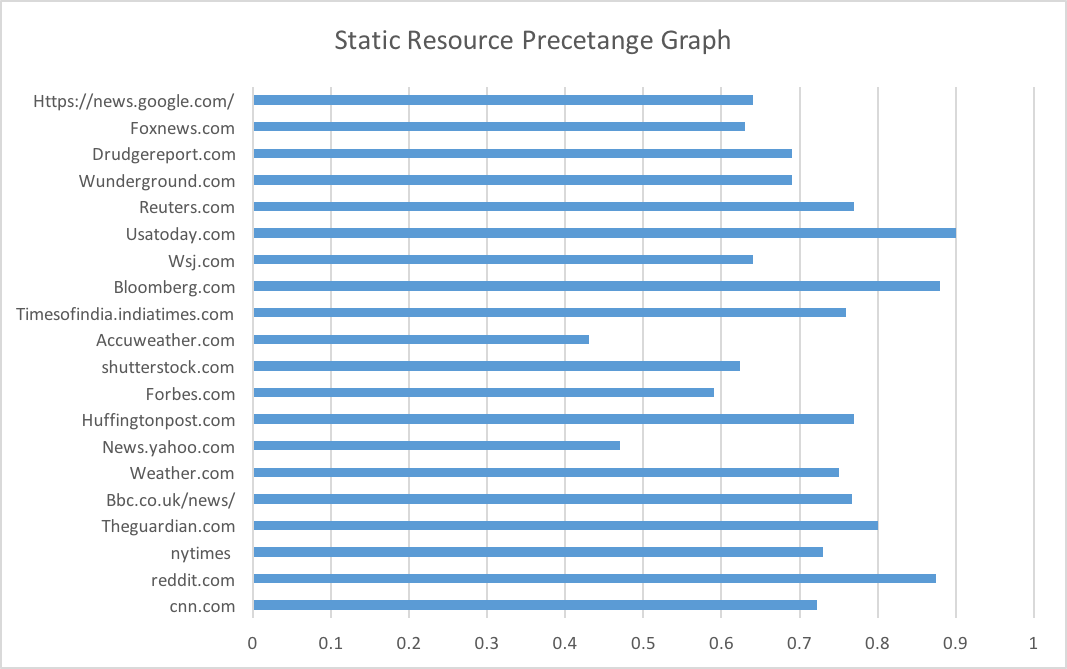
\includegraphics[width=0.5\textwidth]{static_resource_precentage.png}  
	\caption{Percentages of static resources in Alexa's top 20 news websites.}
	\label{fig:static_resource_precentage}
\end{figure} 

In fact, some browsers such as Chrome already have built-in prefetching services based on URL prediction. However, we find that Chrome's prefetching mechanism falls short in the following aspects:
\begin{itemize}
	\item URL Prediction is based on the user's browsing history. If the user clears browsing data, then prediction cannot happen, which means no web resources can be preloaded.
	\item The set of URLs eligible to be prefetched is too conservative, compared with the URLs that the user has typed in the address bar before. Only a small number of websites that are visited most frequently can be prefetched by Chrome.
	\item When a URL is predicted, the majority of the web resources associated with that URL will be preloaded, regardless of the user's need. For that reason, the cost of prefetching unneeded web resources will be huge if Chrome predicts the URL incorrectly, especially when the network bandwidth is limited.
\end{itemize}

We develop AccWeb, a prefetching service with good performance while dealing with the above drawbacks of Chrome. AccWeb runs in 3 separate stages.
\begin{enumerate}
	\item Analyzing. In this stage, AccWeb fetches and records all static web resources of URLs that the user has already visited in the past.
	\item Predicting. Based on the user's typing and browsing history, AccWeb predicts the URL that the user currently tries to navigate (if the prediction confidence is high enough) given the user's current input in the address bar.
	\item Prefetching. After receiving the predicted webpage, The URLs of the web resources on that page are sent through the HTTP link header field to the browser, and the browser starts to preload these resources.
\end{enumerate}
%The second stage is predicting. Based on the user's typing and browsing history, AccWeb predicts the URL that the user currently tries to navigate (if the prediction confidence is high enough) given the user's current input in the address bar.
%The third stage is prefetching. After receiving the predicted webpage, The URLs of the web resources on that page are sent through the HTTP link header field to the browser, and the browser starts to preload these resources.
The demo of AccWeb can be found at \href{https://github.com/caiqizhe/COS561_final_project}{this link}.

AccWeb eliminates (or at least alleviates) the abovementioned drawbacks of Chrome. First, the user's browsing history is stored in a browser extension called Predictor, so flushing browser history in the browser does not affect prefetching in AccWeb. Second, we design a prediction mechanism that is less conservative than Chrome's, while ensuring a high confidence level. Third, we allow the users to have control over which kinds of resources to be prefetched. Note that different users may have different preferences regarding web performance: some users like to load images as quickly as possible, while others care more about the loading time of texts. In addition, under poor network condition, users might want to limit the prefetching service to lower the cost of wrong predictions and to save bandwidth. We implement different modes (e.g. full mode, limited mode, image mode, etc.) that users can select based on their preferences and network condition.


